\documentclass{mathnotes}
\usepackage{mathnotes}

\newcommand{\theauthor}{Guillermo Ruiz Álvarez}
\newcommand{\thetitle}{Ecuaciones Diferenciales Ordinarias}

\title{\thetitle}
\author{\theauthor}
\date{Curso 2013 - 2014\\Universidad Autónoma de Madrid}

\begin{document}

\section{Ecuaciones lineales de orden superior}

\subsection{Problemas lineales con coeficientes constantes}
\label{secEcHomoLinealConstante}
En el caso homogéneo, en el que tenemos una EDO

\[ y^{n)} + a_{n-1}y^{n-1)} + \dotsb + a_1y' + a_0 y = 0 \]

como ya hemos visto anteriomente, podemos obtener el polinomio característico

\[ λ^n + a_{n-1}λ^{n-1} + \dotsb + a_1λ + a_0 = 0 \]

con cuya resolución obtenemos las soluciones asociadas a cada una de las raíces. Podemos tener varias opciones.

\begin{itemize}
\item Si $λ_0$ es una raíz simple, entonces una solución es $y_0(t) = e^{λ_0t}$.
\item Si $λ_1$ es una raíz con multiplicidad $k$, por el método de variación de las constantes encontraremos $k$ soluciones de la forma $t^ie^{λ_1t}$ para $i=0,\hdots,k-1$.
\item En el caso de que la solución sea una raíz compleja, combinamos linealmente soluciones para obtener soluciones reales.
Supongamos que $a+bi$ es una raíz compleja, entonces tenemos que $a-bi$ (por ser el conjugado) también es una raíz del polinomio. A partir de aquí tenemos las soluciones complejas \begin{equation}
\left\lbrace \begin{array}{l}
e^{(a+ib)t} = e^{at}(cos(bt)+isin(bt))\\
e^{(a-ib)t} = e^{at}(cos(bt)-isin(bt))\\
\end{array}\right. 
\end{equation}
de donde obtenemos las soluciones reales haciendo las combinaciones
$$\begin{array}{c|c}
Re(z) = \frac{z+\bar{z}}{2} & Im(z) = \frac{z-\bar{z}}{2i}
\end{array}$$
\end{itemize}

Veamos algunos ejemplos.

\paragraph{Sistema masa-resorte}

Consideramos el siguiente sistema (figura \ref{imgMasaResorte1}), sin rozamiento ni fuerzas externas.

\begin{figure}[hbtp]
\centering
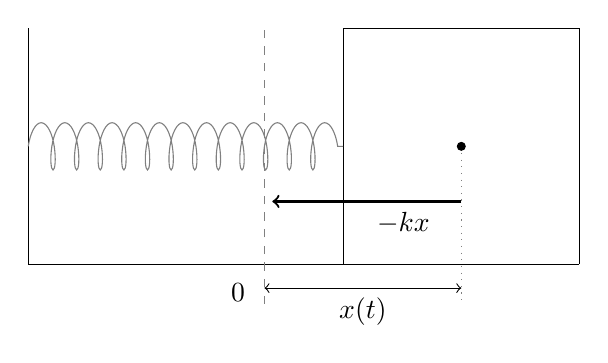
\begin{tikzpicture}
\draw[-] (0,0) -- (7,0);
\draw[-] (0,0) -- (0,3);

\draw[-] (4,0) -- (4,3) -- (7,3) -- (7,0);

\draw[gray,dashed] (3,-0.5) -- (3,3);
\draw[gray,dotted] (5.5,1.5) -- (5.5,-0.5);
\draw[thick,->] (5.5,0.8) -- node[below right, fill=white] {$-kx$} (3.1,0.8);
\node[label=below left:{$0$}] at (3,0) {};

\draw[gray,decoration={aspect=0.3, segment length=3mm, amplitude=3mm,coil},decorate] (0,1.5) -- (4,1.5);

\draw[<->] (3,-0.3) -- node[below] {$x(t)$} (5.5,-0.3);
\node[draw, fill=black, circle, inner sep=1pt] at (5.5,1.5) {};
\end{tikzpicture}
\caption{Sistema masa-resorte, con la fuerza del muelle $-kx$.}
\label{imgMasaResorte1}
\end{figure}

Según la ley de Hooke, la fuerza será

\[ F = -kx \]

donde $k$ es una constante que depende del muelle. Por lo tanto, la ecuación que describe el movimiento es 

\[ mx'' = -kx \]

Podemos transformarla a un problema en derivadas ordinarias

\begin{align*}
x'' + \frac{k}{m}x = 0
x(0) = x_0
x'(0) = v_0
\end{align*}

para el que necesitaremos posición y velocidad iniciales. 

El polinomio característico es

\[ λ^2 + \frac{k}{m} = 0 \]

cuyas raíces son 

\[ λ=\pm \i\sqrt{\frac{k}{m}} \]

Las soluciones complejas son, por lo tanto,

\begin{gather*}
z_1 = e^{\i t\sqrt{\frac{k}{m}}} = \cos \sqrt{\frac{k}{m}} t + \i \sin \sqrt{\frac{k}{m}} t \\
z_1 = e^{-\i t\sqrt{\frac{k}{m}}} = \cos \sqrt{\frac{k}{m}} t - \i \sin \sqrt{\frac{k}{m}} t 
\end{gather*}

Combinándolas de forma lineal, obtenemos dos soluciones reales:

\begin{gather*}
x_1(t) = \Re z_1 = \cos \sqrt{\frac{k}{m}} t \\
x_2(t) = \Im z_1 = \sin \sqrt{\frac{k}{m}} t
\end{gather*}

Aunque se ve a simple vista que esas dos soluciones son independientes (son coseno y seno), deberíamos calcular el wronskiano para comprobar que son realmente independientes.

La solución general nos queda

\begin{equation}\label{eqMasaResorte} x(t) = A\cos \sqrt{\frac{k}{m}} t + B \sin \sqrt{\frac{k}{m}} 
\end{equation}

Las constantes $A$ y $B$ se tendrán que obtener una vez dados los valores iniciales. Si suponemos $x(0) = x_0$, $x'(0) = v_0$, tenemos que

\begin{gather*}
x_0 = x(0) = A \\
x'(t) = -x_0 \sqrt{\frac{k}{m}} \sin \sqrt{\frac{k}{m}} t + B \sqrt{\frac{k}{m}}\cos\sqrt{\frac{k}{m}} t \\
v_0 = x'(0) = B \sqrt{\frac{k}{m}} \\
B = \frac{v_0}{\sqrt{\frac{k}{m}}}
\end{gather*}

Si bien esta solución está perfectamente bien, los físicos son gente rara y prefieren hacer otra cosa. Reescriben el punto $(A,B)$ en coordenadas polares, de tal forma que

\begin{align*}
A &= R\cos φ \\
B &= R\sin φ 
\end{align*}

Sustituyendo en \eqref{eqMasaResorte}

\[ x(t) = R\left(\cos \sqrt{\frac{k}{m}} t\cos φ + \sin \sqrt{\frac{k}{m}} t \sin φ \right) = R\cos\left(\sqrt{\frac{k}{m}}t - Φ\right) \]

donde $Φ = \arctan \frac{B}{A}$ es el desfase, que actúa de velocidad inicial del sistema.

\paragraph{Sistema masa-resorte con rozamiento}

Replanteemos el problema anterior con rozamiento.
\begin{figure}
\centering
\begin{tikzpicture}
\draw[-] (0,0) -- (7,0);
\draw[-] (0,0) -- (0,3);

\draw[-] (4,0) -- (4,3) -- (7,3) -- (7,0);

\draw[gray,dashed] (3,-0.5) -- (3,3);
\draw[gray,dotted] (5.5,1.5) -- (5.5,-0.5);
\draw[thick,->] (5.5,2) -- node[above right, fill=white] {$-εx'$} (2.7,2);
\draw[thick,->] (5.5,0.8) -- node[below right, fill=white] {$-kx$} (3.1,0.8);
\node[label=below left:{$0$}] at (3,0) {};

\draw[gray,decoration={aspect=0.3, segment length=3mm, amplitude=3mm,coil},decorate] (0,1.5) -- (4,1.5);

\draw[<->] (3,-0.3) -- node[below] {$x(t)$} (5.5,-0.3);
\node[draw, fill=black, circle, inner sep=1pt] at (5.5,1.5) {};
\end{tikzpicture}
\caption{Sistema masa-resorte con rozamiento (fuerza $-εx'$).}
\end{figure}

La ecuación cambia al añadir el rozamiento:

\begin{gather} mx'' = -kx - εx' \nonumber \\
x'' + \frac{ε}{m}x' + \frac{k}{m}x = 0
\end{gather}

Resolvemos el polinomio característico \[ λ^2 + \frac{ε}{m}λ + \frac{k}{m} = 0 \] y nos queda

\[ λ = \frac{-ε}{2m} \pm \sqrt{\left(\frac{ε}{2m}\right)^2 - \frac{k}{m}} \].

Tenemos que plantear tres casos basados en el valor de $Δ =\left(\frac{ε}{2m}\right)^2 - \frac{k}{m}$: si es mayor, igual o menor que cero.

\subparagraph{Primer caso: $Δ > 0$ (rozamiento alto)}

Tenemos 

\begin{gather*}
λ_+ = \frac{-ε}{2m} + \sqrt{\left(\frac{ε}{2m}\right)^2 - \frac{k}{m}} \\
λ_- = \frac{-ε}{2m} - \sqrt{\left(\frac{ε}{2m}\right)^2 - \frac{k}{m}} 
\end{gather*}

De sus expresiones vemos que tanto $λ_+$ como $λ_-$ son negativos. La solución general del problema es 

\( x(t) = Ae^{λ_+t} + Be^{λ_-t} \)

Despejando de los valores iniciales $x(0) = x_0$, $x'(0) = v_0$ y haciendo cuentas,

\[ x(t) = \frac{1}{λ_+ - λ_-}\left((v_0-λ_-x_0)e^{λ_+t} - (v_0-λ_+x_0)e^{λ_-t}\right) \]

De esa ecuación vemos que, cuando $t\to ∞$, $x(t) \to 0$. Es decir, el objeto tiende a pararse.

También querríamos ver cuántas veces pasamos por la posición de equilibrio. Tenemos que resolver la ecuación

\[ e^{(λ_+ - λ_-)t} = \frac{v_0-λ_+x_0}{v_0-λ_-x_0} \]

que no tiene solución. Por lo tanto, el objeto no llega nunca a la posición de equilibrio.

\subparagraph{Segundo caso: $Δ=0$}

En este caso, tenemos $λ=\frac{-ε}{2m}$ que es una raíz doble. Por el método de variación de las constantes, nuestras dos soluciones son

\[ x_1(t) = e^{\frac{-ε}{2m}t};\quad x_2(t) = te^{\frac{-ε}{2m}t} \]

y la solución general se expresa como 

\( x(t) = A e^{\frac{-ε}{2m}t} + B t e^{\frac{-ε}{2m}t} = e^{\frac{-ε}{2m}t} \left(A + Bt\right) \)

Al igual que en el anterior caso, $x(t) \convs[][t][∞] 0$, pero aquí $x(t) = 0$ sí que podemos tener soluciones.

\subparagraph{Tercer caso: $Δ < 0$ (sin rozamiento)}

Aquí tendremos raíces complejas, es decir:

\[ λ_+ = \frac{-ε}{2m} + \i \sqrt{\frac{k}{m} - \left(\frac{ε}{2m}\right)^2} \]

y su conjugada. De esta forma, las dos soluciones reales serán

\begin{gather*}
x_1(t) = e^{\frac{-ε}{2m}t} \cos t\sqrt{\frac{k}{m} - \left(\frac{ε}{2m}\right)^2} \\
x_1(t) = e^{\frac{-ε}{2m}t} \sin t\sqrt{\frac{k}{m} - \left(\frac{ε}{2m}\right)^2} \\
\end{gather*}

Podemos extraer la solución general y hacer el cambio del anterior apartado, pasando a polares $(A,B) \sim (R\cos φ, R\sin φ)$s, de tal forma que nos queda la solución general

\( x(t) = R e^{-\frac{ε}{2m}t} \cos \left(t\sqrt{\frac{k}{m} - \left(\frac{ε}{2m}\right)^2} - Φ\right) \)

Es decir, hay un decaimiento exponencial de la amplitud. La gráfica de la función sería la de la figura \ref{imgMasaResorteSeno}

\easyimg{img/MasaResorteSeno.png}{$x(t)$ para un sistema masa-resorte}{imgMasaResorteSeno}

\paragraph{Péndulo simple}

Consideramos un péndulo simple sin rozamiento.

\begin{figure}[hbtp]
\centering
\begin{tikzpicture}
\draw[-] (-2,0) -- (2,0);
\draw[-] (0,1) -- (0,-4);

\draw[-] (0,0) -- (1,-2);
\draw[->] (1,-2) -- node[right] {$mg$} (1,-3.5);
\node[draw, fill=white, circle, inner sep=4pt] at (1,-2) {};
\end{tikzpicture}
\caption{El péndulo}
\end{figure}

Tenemos las ecuaciones de posición

\[ σ(t) = (L\sin θ(t), - L \cos θ(t))\]

, de velocidad

\[ σ'(t) = (Lθ'(t)\cos θ(t), Lθ'(t)\sin θ(t))\]

y aceleración

\begin{align*}
 σ''(t) = (&-L(θ'(t))^2\sin(t) + Lθ''(t)\cos(t), \\
 & L(θ'(t))^2\cos θ(t) + Lθ''(t)\sin θ(t) 
 \end{align*}.
 
Dividimos en la componente tangencial y la perpendicular a la cuerda. Igualando algo

\[ mg( -\cosθ, -\sin θ)\sin θ  = m σ''(t) \]

y por lo tanto nos quedan las dos ecuaciones
\[ 
\left\{\begin{matrix}
 -g\sin θ \cos^2 θ = -L θ'^2 \cos θ \sin θ+ Lθ''\cos^2θ  \\
 -g\sin θ \sin^2 θ = -L θ'^2 \sin θ \cos θ  + Lθ''\sin^2θ  
 \end{matrix}\right\} \]
 
 La ecuación final es \[ -g\sin θ = L θ'' \] o, transformada 
 
 \[ θ'' + \frac{g}{L} \sin θ = 0 \]

Por Taylor, podemos aproximar $\sin θ \sim θ$ cuando θ es pequeña, de tal forma que nos reducimos al caso de un sistema masa-resorte.



\end{document}